\documentclass[a4paper]{article}
\usepackage{graphicx}
\usepackage[left=3.18cm, right=3.18cm, top=2.54cm, bottom=2.54cm]{geometry}
\usepackage{fancyhdr}
\usepackage{setspace}
\usepackage{amsmath}
\usepackage{amssymb}
\usepackage{booktabs}
\usepackage{colortbl}
\usepackage{xcolor}

\newcommand{\minval}[1]{\textbf{\textcolor{red}{#1}}}

\pagestyle{fancy}
\lhead{} % Clear left header
\chead{ESE5004 - Final Report} % Center header
\rhead{} % Clear right header
\onehalfspacing
\setlength{\parindent}{0pt}
\setlength{\parskip}{1em}

\begin{document}
\begin{titlepage}
    \centering
    \vspace*{-2.5cm}
    
\includegraphics[width=0.75\textwidth]{../attachment/nus.jpg} \\
    \Huge
    \textbf{Final Report}

    \vspace{1.5cm}
    \Large
    \textbf{Topic:} Application of Supervised Learning Methods to Transformation Mechanisms in DBPs Formation in simulated drinking water distribution network

    \vspace{1.5cm}
    \textbf{Name:} Zhou Dafu \\
    \textbf{Number:} A0331761J

    \vspace{1cm}
    \textbf{Supervisor:} Prof. Hu Jiangyong \\
    \textbf{Mentor:} Mr. Sun Yuanpeng

    \vfill
    \Large
    \date{\today}
\end{titlepage}

\section{Introduction}

\subsection{Background}
Disinfection is a critical step in municipal water treatment, designed to eliminate pathogenic microorganisms and ensure public health. However, chemical disinfectants, most commonly chlorine, react with naturally occurring organic matter (NOM) and other precursors in the water to form a wide array of unintended compounds known as disinfection by-products (DBPs)~\cite{galliard2004organic}. Many DBPs are of health concern due to their potential carcinogenic and mutagenic properties~\cite{siddique2012review}. Consequently, water utilities face the challenge of balancing microbial safety with the minimization of DBP formation.

Predicting DBP concentrations within complex water distribution systems (WDS) is a significant challenge due to dynamic hydraulic conditions and complex chemical kinetics. Traditional monitoring relies on infrequent grab sampling and laboratory analysis, which is costly and provides low temporal resolution. This research aims to leverage high-frequency sensor data and supervised machine learning techniques to develop predictive models for DBP indicators, such as Total Residual Chlorine (TRC), Total Organic Carbon (TOC), and pH. The successful development of these models would enable proactive operational control to mitigate DBP formation and improve water quality management. This report outlines the progress made in data preprocessing, model selection, and experimental design for this purpose.

\subsection{DBP Formation Chemistry}
The formation of Disinfection By-Products (DBPs) in this system is a multi-step process governed by the interactions between disinfectants and precursors under alkaline conditions. The process begins with the formation of monochloramine ($NH_2Cl$), which serves as the primary disinfectant. In the presence of ammonium ions ($NH_4^+$) and hypochlorite ions ($OCl^-$), which are the dominant species in the alkaline environment created by slaked lime, monochloramine is produced according to the following total reaction:
\begin{equation}
    \text{NH}_3 + \text{OCl}^- \rightarrow \text{NH}_2\text{Cl} + \text{OH}^-
\end{equation}
Once formed, chloramines can react with organic nitrogen precursors (e.g., secondary amines) present in the water. This reaction typically involves the formation of intermediate compounds, such as chlorinated unsymmetrical dialkylhydrazines. These intermediates are subsequently oxidized by dissolved oxygen to form nitrogenous DBPs (N-DBPs), such as nitrosamines (e.g., N-nitrosodimethylamine, NDMA)~\cite{hua2015formation}. This pathway highlights the critical role of chloramine speciation and the presence of organic precursors in the generation of potentially harmful by-products.

\subsection{Deep Learning and Machine Learning in Water Engineering}
Deep learning and advanced machine learning models have emerged as powerful tools in water engineering, offering new capabilities for modeling complex, non-linear systems that are difficult to capture with traditional mechanistic models. In the context of water quality, these models can leverage high-frequency sensor data to predict critical parameters, detect anomalies, and optimize treatment processes~\cite{zhang2020review}. This study aims to bridge the gap between traditional water chemistry and modern data-driven approaches by applying various machine learning architectures to the problem of DBP prediction.

\subsection{Gradient Boosting Decision Trees (GBDT)}
Gradient Boosting Decision Trees (GBDT) are a class of powerful ensemble learning algorithms that build a series of decision trees sequentially, with each new tree attempting to correct the errors made by the previous ones.
\begin{itemize}
    \item \textbf{XGBoost (Extreme Gradient Boosting):} XGBoost~\cite{chen2016xgboost} improves upon traditional gradient boosting by incorporating second-order derivative approximations and L1/L2 regularization to prevent overfitting, making it highly robust and efficient.
    \item \textbf{LightGBM:} LightGBM~\cite{ke2017lightgbm} uses a histogram-based algorithm and a leaf-wise tree growth strategy, making it exceptionally fast and capable of handling large-scale data with lower memory consumption.
    \item \textbf{CatBoost:} CatBoost~\cite{prokhorenkova2018catboost} is specifically designed to handle categorical features automatically without explicit preprocessing (e.g., one-hot encoding) and uses oblivious trees to reduce overfitting and enhance inference speed.
\end{itemize}

\begin{figure}[h!]
    \centering
    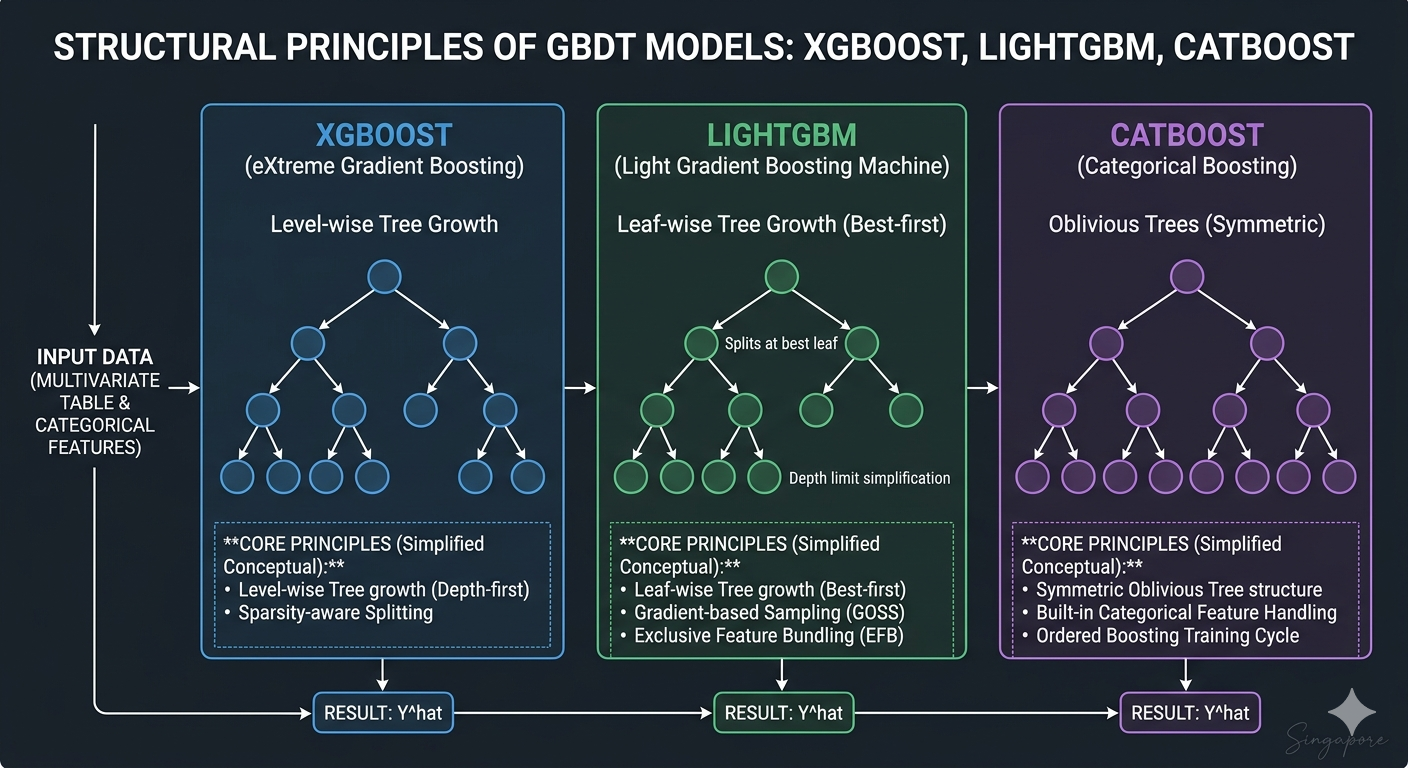
\includegraphics[width=0.75\textwidth]{../attachment/3GBDTs.png}
    \caption{Conceptual comparison of the three GBDT models.}
    \label{fig:gbdts}
\end{figure}

\subsection{Neural Network Architectures}
To capture the complex, non-linear dynamics of DBP formation, several classical and novel neural network architectures are considered for this regression task, as illustrated sequentially below:

\begin{itemize}
    \item \textbf{Multilayer Perceptron (MLP):} A foundational feedforward neural network that can model complex non-linear relationships. It consists of an input layer, one or more hidden layers, and an output layer. Each layer contains neurons that are fully connected to the neurons in the subsequent layer. In addition to accepting single data points as input, the MLP architecture in this study was also adapted to process time-series data by flattening a fixed-length window of historical time-series data into a single vector, which is then fed into the network. This allows the MLP to capture some temporal patterns without recurrent connections.
    
    \item \textbf{Recurrent Neural Network (RNN):} Designed to handle sequential data by maintaining a hidden state that captures past information. The output at a given time step is a function of the current input and the hidden state from the previous time step. This recurrent connection allows RNNs to model temporal dependencies, but they can struggle with long-term dependencies due to the vanishing gradient problem.
    
    \item \textbf{Long Short-Term Memory (LSTM):} A specialized RNN architecture that uses gating mechanisms (input, forget, and output gates) to overcome the vanishing gradient problem and effectively learn long-term dependencies~\cite{hochreiter1997long}. The gates control the flow of information, allowing the network to selectively remember or forget information over long sequences, making it well-suited for time-series forecasting.
    
    \item \textbf{Gated Recurrent Unit (GRU):} A simplified version of the LSTM with fewer parameters, which often performs comparably on many tasks. It combines the input and forget gates into a single "update gate" and merges the cell state and hidden state. This makes the GRU more computationally efficient than the LSTM while still retaining its ability to capture long-term dependencies.
    
    \item \textbf{Transformer (Encoder-Only):} Originally designed for Natural Language Processing (NLP), the Transformer architecture utilizes a multi-head self-attention mechanism. In the context of time-series analysis, this self-attention mechanism calculates attention weights across the entire sequence simultaneously, allowing the model to capture global temporal dependencies and long-range correlations dynamically, independent of their distance~\cite{vaswani2017attention}. Unlike traditional NLP tasks (such as machine translation) that typically require a full Encoder-Decoder structure to generate an output sequence of variable length, this predictive regression task utilizes an Encoder-Only architecture. Because the goal is to map a fixed-length historical multi-variate input to a specific set of concurrent continuous numerical values without auto-regressive sequential generation, omitting the Decoder significantly improves computational efficiency and reduces overfitting while retaining the model's robust feature extraction capabilities.
    
    \item \textbf{Mamba:} Mamba represents a novel class of state-space models (SSMs) that achieve linear time complexity for sequence modeling while offering hardware-aware optimizations. It selectively filters and retains information over long sequences, providing an efficient alternative to the computationally expensive attention mechanism in Transformers~\cite{gu2023mamba}.
\end{itemize}

\begin{figure}[h!]
    \centering
    \includegraphics[width=0.75\textwidth]{../attachment/mlp.png}
    \caption{Structure of a Multilayer Perceptron.}
    \label{fig:mlp_structure}
\end{figure}

\begin{figure}[h!]
    \centering
    \includegraphics[width=0.75\textwidth]{../attachment/rnn.png}
    \caption{Structure of a Recurrent Neural Network.}
    \label{fig:rnn_structure}
\end{figure}

\begin{figure}[h!]
    \centering
    \includegraphics[width=0.75\textwidth]{../attachment/lstm.png}
    \caption{Structure of a Long Short-Term Memory Cell.}
    \label{fig:lstm_structure}
\end{figure}

\begin{figure}[h!]
    \centering
    \includegraphics[width=0.75\textwidth]{../attachment/gru.png}
    \caption{Structure of a Gated Recurrent Unit Cell.}
    \label{fig:gru_structure}
\end{figure}

\begin{figure}[h!]
    \centering
    
\includegraphics[width=0.75\textwidth]{"../attachment/transformer from Attention Is All You Need.png"}
    \caption{Transformer Architecture.}
    \label{fig:transformer_structure}
\end{figure}

\begin{figure}[h!]
    \centering
    
\includegraphics[width=0.75\textwidth]{"../attachment/ssm from Mamba: Linear-Time Sequence Modeling with Selective State Spaces.png"}
    \caption{Mamba Architecture.}
    \label{fig:mamba_structure}
\end{figure}

\subsection{Fine-Tuning and Transfer Learning}
Transfer learning is a machine learning paradigm where knowledge acquired while solving one problem is applied to a different but related problem. This is particularly valuable when the target dataset is small or slightly shifted, as it allows the model to leverage robust feature representations learned from a vast source dataset. In deep learning, Transfer Learning is primarily implemented through a methodology known as Fine-Tuning, which involves taking a pre-trained model and further training it on the new task. In this study, we utilize fine-tuning to transfer the learned predictive capabilities from the baseline $29^{\circ}\text{C}$ datasets to the $35^{\circ}\text{C}$ datasets. We explore three common fine-tuning strategies:
\begin{itemize}
    \item \textbf{Full Fine-Tuning:} All parameters of the pre-trained model are updated during training on the new task. This provides the most flexibility but risks overfitting on small datasets.
    \item \textbf{Partial Fine-Tuning (Frozen Layers):} The lower layers of the model (often feature extractors) are frozen, and only the top layers (task-specific heads) are trained. This helps retain learned generic representations and speeds up training.
    \item \textbf{Adapter (LoRA):} Low-Rank Adaptation (LoRA)~\cite{hu2021lora} introduces small, trainable bottleneck layers into the frozen pre-trained model. This allows for parameter-efficient fine-tuning while maintaining the expressive power of the original model.
\end{itemize}

\section{Objectives}
The primary objectives of this study are:
\begin{enumerate}
    \item To evaluate the performance of various classical deep learning architectures (MLP, RNN, LSTM, GRU), classical machine learning models (XGBoost, LightGBM, CatBoost), and novel sequence models (Transformer, Mamba) in predicting water quality parameters from sensor data.
    \item To investigate the effectiveness of the Transformer architecture for fine-tuning and transfer learning across datasets with identical format but varying conditions (e.g., different water sources and temperatures).
    \item To investigate the correlation between high-frequency sensor measurements (TRC, pH, TOC, etc.) and DBP formation.
    \item To establish a robust machine learning framework and an interactive GUI application for predicting DBP concentrations based on readily available sensor data, thereby enabling real-time monitoring and control.
\end{enumerate}

\section{Methodology}

\subsection{System Description and Data Acquisition}
The study focuses on a section of a water distribution system comprising five main stages, as illustrated in Figure \ref{fig:reactors}:
\begin{enumerate}
    \item \textbf{Feed Water Tank (FWT):} Raw water storage before post-treatment. Not included in the modeling.
    \item \textbf{Disinfection Tank (DT):} Where disinfection chemicals are introduced and mixed.
    \item \textbf{Retention Tank (RT):} Storage before water supply.
    \item \textbf{Pipeline 1 (PPL1):} Upper stream of distribution network.
    \item \textbf{Pipeline 2 (PPL2):} Lower stream of distribution network.
\end{enumerate}

\begin{figure}[h!]
\centering
\includegraphics[width=0.8\textwidth]{../attachment/reactors.png}
\caption{Schematic of the reactor flow process in the water distribution system.}
\label{fig:reactors}
\end{figure}

Water quality data is collected via multi-parameter sensors at different stages. The parameters include Total Residual Chlorine (TRC), pH, Conductivity, Fluorescent Dissolved Organic Matter (fDOM), Dissolved Oxygen (DO), Total Organic Carbon (TOC), and Dissolved Organic Carbon (DOC). Data is recorded at a 5-minute interval. The availability of sensor measurements at each stage is summarized in Table \ref{tab:sensor_data}.

\begin{table}[h!]
\centering
\caption{Availability of Sensor Measurements at Each Stage}
\label{tab:sensor_data}
\begin{tabular}{lcccc}
\toprule
\textbf{Parameter} & \textbf{DT} & \textbf{RT} & \textbf{PPL1} & \textbf{PPL2} \\
\midrule
TRC & \checkmark & \checkmark & \checkmark & \checkmark \\
pH & \checkmark & \checkmark & \checkmark & \checkmark \\
Conductivity & \checkmark & \checkmark & \checkmark & \checkmark \\
fDOM (QSU) &  & \checkmark & \checkmark & \checkmark \\
DO &  & \checkmark & \checkmark & \checkmark \\
TOC &  & \checkmark & \checkmark & \checkmark \\
DOC &  & \checkmark & \checkmark & \checkmark \\
\bottomrule
\end{tabular}
\end{table}

To comprehensively evaluate the models and transfer learning capabilities, the data is divided into four distinct datasets representing different water sources (CAWW, LSWW) and temperature conditions ($29^{\circ}\text{C}$, $35^{\circ}\text{C}$): \textbf{CAWW\_29}, \textbf{LSWW\_29}, \textbf{CAWW\_35}, and \textbf{LSWW\_35}. The CAWW\_29 dataset serves as the foundational dataset for hyperparameter tuning, training, and comparative evaluation across all machine learning models. The remaining datasets (LSWW\_29, CAWW\_35, LSWW\_35) are utilized subsequently to investigate the performance of different Transformer fine-tuning methodologies.

\subsection{Data Preprocessing}

\subsubsection{Imputation of Missing Values}
A unique challenge in the dataset arises from the measurement setup for PPL1 and PPL2, where a single sensor alternates between the two locations every 30 minutes. This results in blocks of six consecutive missing values for each pipeline stage, alternating with six valid measurements. To create a continuous time series for model training, these missing values must be imputed.

The imputation process is as follows, with a visual representation in Figure \ref{fig:imputation_example}. For a block of missing data with available data segments both before and after, a two-step approach is used. First, linear regression models are fitted to the data segments preceding and succeeding the gap. The initial imputed values are determined by creating a linear interpolation between the predicted value at the end of the preceding segment and the predicted value at the beginning of the succeeding segment. Subsequently, random noise is added to these initial values. The variance of this noise is set to the smaller of the variances from the two fitted linear regression models, preserving the statistical properties of the local time series. In cases where a missing data block is at the beginning or end of the dataset, only the nearest available data segment is used. A linear regression model is fitted to this segment, and the resulting regression line is extrapolated to fill the missing values. Random noise, with a variance equal to that of the regression model, is then added to these extrapolated values.

\begin{figure}[h!]
\centering
\includegraphics[width=0.8\textwidth]{../attachment/imputation.png}
\caption{Conceptual Example of Missing Value Imputation.}
\label{fig:imputation_example}
\end{figure}

\subsubsection{Data Segmentation}
After thoroughly imputing the missing values, the continuous time-series data is directly segmented into appropriate time windows to create input-output pairs. This sliding window approach allows recurrent networks and self-attention mechanisms to learn temporal dependencies inherently. The segmented dataset is subsequently divided into training, validation, and testing sets using a chronological split ratio of 7:1.5:1.5, respectively. This ensures that the models are trained on past data and evaluated on future unseen data, preserving the temporal integrity of the predictive task.

\subsection{Model Training and Evaluation}

All models are systematically trained and evaluated following standard machine learning principles. The process involves feeding the model with input-output pairs and optimizing its internal weights to minimize a loss function, which quantifies the error between the model's predictions and the true values. Figure \ref{fig:training_flowchart} conceptually outlines the model evaluation workflow.

\begin{figure}[h!]
    \centering
    \includegraphics[width=\textwidth]{../attachment/model workflow.png}
    \caption{Model Training and Evaluation Workflow.}
    \label{fig:training_flowchart}
\end{figure}

For the current experimental framework, the \textbf{CAWW\_29} dataset is primarily used to conduct a rigorous comparison of different models. 
\begin{itemize}
    \item \textbf{Input Variables:} All available sensor variables from the upstream Disinfection Tank (DT) and Retention Tank (RT) serve as input features.
    \item \textbf{Output Variables:} The goal is to perform direct regression on the corresponding absolute concentration values at Pipeline 1 (PPL1) and Pipeline 2 (PPL2).
\end{itemize}

\textbf{Modeling Strategies:}
Because GBDT models (XGBoost, LightGBM, CatBoost) are natively designed for single-output regression tasks, individual models are trained separately for each specific output target at PPL1 and PPL2. Conversely, the deep neural network architectures inherently support multi-output configurations; thus, a single unified neural network is trained to simultaneously predict all target variables across PPL1 and PPL2.

The foundational principles applied during the training phase include:
\begin{itemize}
    \item \textbf{Loss Function:} Mean Squared Error (MSE) is chosen as the primary loss function, suitable for penalizing larger errors in regression tasks.
    \item \textbf{Optimization:} The Adam optimizer~\cite{kingma2014adam}, an adaptive learning rate optimization algorithm, is used to update the neural network weights via backpropagation. For GBDT models, built-in gradient-based optimization algorithms are natively utilized.
    \item \textbf{Dataset Splitting:} As outlined previously, the chronological data is split into training (70\%), validation (15\%), and test (15\%) sets. The model learns from the training set, its hyperparameters are tuned based on performance on the validation set, and its final performance is evaluated on the unseen test set.
    \item \textbf{Regularization:} To prevent overfitting, techniques like Dropout~\cite{srivastava2014dropout} are extensively used in neural networks. Additionally, an early stopping mechanism is implemented across all models: training is halted if the validation loss does not improve for a specified number of epochs, and the model with the best validation performance is saved.
\end{itemize}

\subsection{Hyperparameter Optimization}
The performance of machine learning models is highly sensitive to the choice of hyperparameters. Key hyperparameters include learning rate, batch size, dropout rate, number of layers, number of units per layer, and the history length for sequential models. While methods like grid search and random search~\cite{bergstra2012random} exist, this project employs \textbf{Bayesian Optimization}~\cite{snoek2012practical}. Bayesian optimization builds a probabilistic model of the objective function (e.g., validation loss) and uses it to intelligently select the most promising hyperparameters to evaluate next. This approach is more efficient than exhaustive or random searches, often finding better hyperparameter configurations in fewer iterations.

\subsection{Transformer Fine-Tuning Strategy}
To investigate the transferability of the learned dynamics, a fine-tuning strategy was designed exclusively using the Transformer architecture. The Transformer was selected because of its overwhelming dominance in Large Language Models (LLMs), indicating its superior capability to grasp contextual and sequential patterns. Moreover, its attention-driven architecture is highly amenable to modern parameter-efficient fine-tuning paradigms like LoRA and partial freezing.

\textbf{Experimental Flow:}
\begin{enumerate}
    \item Extract the best hyperparameter configuration found via Bayesian Optimization for the Transformer on the \textbf{CAWW\_29} dataset.
    \item Train a new Transformer from scratch on the \textbf{LSWW\_29} dataset using these optimal hyperparameters. This provides established base models for the two distinct water sources at the $29^{\circ}\text{C}$ baseline.
    \item Fine-tune the pre-trained \textbf{CAWW\_29} model on the \textbf{CAWW\_35} dataset utilizing three methods: Full Fine-Tuning, Partial Fine-Tuning (freezing the encoder), and Adapter.
    \item Concurrently, fine-tune the \textbf{LSWW\_29} model on the \textbf{LSWW\_35} dataset using the same three methods.
\end{enumerate}

\begin{figure}[h!]
    \centering
    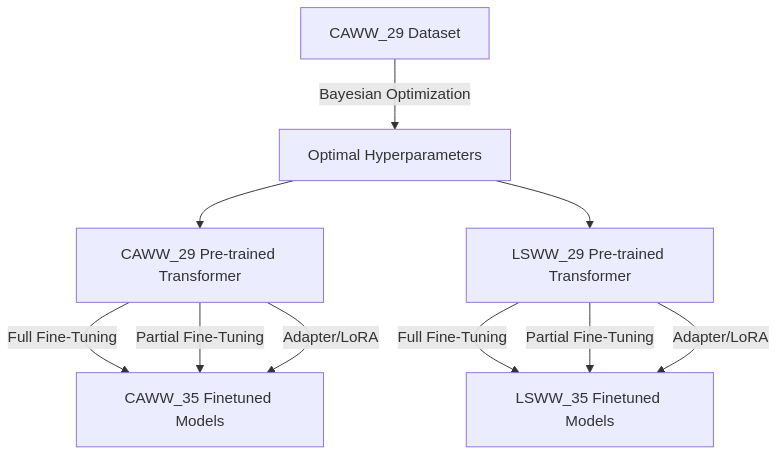
\includegraphics[width=0.8\textwidth]{../attachment/finetuning_workflow.png}
    \caption{Experimental workflow diagram for Transformer Fine-Tuning across datasets.}
    \label{fig:finetuning_workflow}
\end{figure}

This decoupled approach ensures that major chemical composition differences between different water sources (CAWW vs. LSWW) are independently addressed through separate baseline training, while the reaction kinetic changes driven by temperature variations ($29^{\circ}\text{C}$ to $35^{\circ}\text{C}$) are isolated and efficiently learned via fine-tuning techniques.

\section{Results}
All model training, fine-tuning, and evaluation processes were conducted on a high-performance workstation running the Fedora 43 operating system, equipped with an NVIDIA GeForce RTX 4070 GPU. This hardware acceleration ensured efficient computation, particularly for the self-attention mechanisms of the Transformer and the recurrent states of deep neural networks.

To quantitatively evaluate the performance of our regression models, we utilize four fundamental statistical metrics: Mean Squared Error (MSE), Mean Absolute Error (MAE), Root Mean Squared Error (RMSE), and the Coefficient of Determination ($R^2$). 
\begin{align*}
    \text{MSE} &= \frac{1}{n} \sum_{i=1}^{n} (y_i - \hat{y}_i)^2 \\
    \text{MAE} &= \frac{1}{n} \sum_{i=1}^{n} |y_i - \hat{y}_i| \\
    \text{RMSE} &= \sqrt{\text{MSE}} \\
    R^2 &= 1 - \frac{\sum (y_i - \hat{y}_i)^2}{\sum (y_i - \bar{y})^2}
\end{align*}
For the multi-output neural networks, the reported MSE is the aggregated mean loss across all predicted target variables. Although models were trained to predict a multitude of parameters across PPL1 and PPL2, the visual demonstrations in the subsequent sections will focus exclusively on the prediction of Total Residual Chlorine at Pipeline 2 (\textbf{TRC-PPL2}) as a representative, critical metric.

\subsection{GBDT Models Results}

Table \ref{tab:gbdt_metrics} summarizes the predictive performance of the three GBDT models on the CAWW\_29 dataset.

\begin{table}[h!]
\centering
\caption{Overall Performance Metrics for GBDT Models (CAWW\_29)}
\label{tab:gbdt_metrics}
\begin{tabular}{lcccc}
\toprule
\textbf{Model} & \textbf{MSE} & \textbf{MAE} & \textbf{RMSE} & \textbf{R²} \\
\midrule
\textbf{XGBoost} & \textbf{0.221734} & \textbf{0.192014} & \textbf{0.470886} & \textbf{0.999976} \\
LightGBM & 0.866635 & 0.401697 & 0.930932 & 0.999905 \\
CatBoost & 2.057596 & 0.628809 & 1.434432 & 0.999775 \\
\bottomrule
\end{tabular}
\end{table}

Due to space constraints, the detailed visualized Prediction vs. True plots and Y=X Scatter plots for the GBDT models are provided in Appendix \ref{app:visualizations} (Table \ref{tab:gbdt_plots}).

\textbf{Analysis:} XGBoost demonstrated the most superior performance among the tree-based models. However, despite their ease of use, traditional machine learning models like GBDTs possess inherent limitations compared to Deep Learning when dealing with complex time-series regression tasks:
\begin{itemize}
    \item \textbf{Lack of Representation Learning:} GBDTs cannot automatically extract hierarchical representations from raw data, heavily relying on manual feature engineering.
    \item \textbf{Poor on Unstructured Data:} They struggle to capture spatial or temporal dependencies naturally.
    \item \textbf{Axis-Aligned Decision Boundaries:} GBDTs split features orthogonally, resulting in discrete, non-smooth step-like predictions.
    \item \textbf{Weak Extrapolation:} Tree models cannot predict numerical values beyond the bounds of the training data.
    \item \textbf{Non-Differentiable:} The discrete nature of tree splits makes them incompatible with end-to-end gradient-based optimization in larger systems.
    \item \textbf{Low Scaling Ceiling:} Performance plateaus relatively quickly, lacking the exponential scaling laws seen in massive Neural Networks.
\end{itemize}

\subsection{Neural Network Models Results}

Table \ref{tab:nn_metrics} presents the consolidated results for the six Neural Network architectures evaluated on the CAWW\_29 dataset.

\begin{table}[h!]
\centering
\caption{Overall Performance Metrics for Neural Network Models (CAWW\_29)}
\label{tab:nn_metrics}
\begin{tabular}{lcccc}
\toprule
\textbf{Model} & \textbf{MSE} & \textbf{MAE} & \textbf{RMSE} & \textbf{R²} \\
\midrule
MLP & 0.238894 & 0.204610 & 0.488768 & 0.999974 \\
RNN & 0.425535 & 0.267785 & 0.652331 & 0.999953 \\
GRU & 0.200362 & 0.192114 & 0.447619 & 0.999978 \\
\textbf{LSTM} & \textbf{0.177875} & \textbf{0.173571} & \textbf{0.421752} & \textbf{0.999981} \\
Transformer & 0.420845 & 0.278945 & 0.648726 & 0.999954 \\
Mamba & 0.816778 & 0.384420 & 0.903757 & 0.999911 \\
\bottomrule
\end{tabular}
\end{table}

The extensively visualized performance plots (Prediction vs. True and Y=X Scatter plots) for all six Neural Network architectures are structurally detailed in Appendix \ref{app:visualizations} (Tables \ref{tab:nn_plots_1} and \ref{tab:nn_plots_2}) to maintain the reading flow of this section.

\textbf{Analysis:} The LSTM model exhibited the highest predictive accuracy across all metrics for the time-series regression of the multiple target variables. While the novel architectures like Transformer and Mamba yielded sub-optimal results on this specific, relatively short-sequence dataset compared to LSTM, they still remain highly valuable and are considered the mainstream future trajectory of deep learning research. The Transformer's global attention mechanism becomes significantly more potent when sequences grow extremely long and structural complexity increases, a domain where RNN/LSTM typically fail. Furthermore, the Transformer architecture facilitates seamless fine-tuning and parameter-efficient post-training updates, making it a critical asset for adaptable systems.

\subsection{Fine-Tuning Results}

We evaluated the transfer learning capabilities of the Transformer model by Fine-Tuning the pre-trained CAWW\_29 and LSWW\_29 models on the CAWW\_35 and LSWW\_35 datasets, respectively. Table \ref{tab:finetune_metrics} demonstrates the performance of the Full, Partial, and Adapter fine-tuning approaches.

\begin{table}[h!]
\centering
\caption{Fine-Tuning Performance on $35^{\circ}\text{C}$ Datasets}
\label{tab:finetune_metrics}
\begin{tabular}{l|cccc|cccc}
\toprule
\textbf{Method} & \multicolumn{4}{c|}{\textbf{CAWW\_35}} & \multicolumn{4}{c}{\textbf{LSWW\_35}} \\
& \textbf{MSE} & \textbf{MAE} & \textbf{RMSE} & \textbf{R²} & \textbf{MSE} & \textbf{MAE} & \textbf{RMSE} & \textbf{R²} \\
\midrule
\textbf{Full} & \textbf{0.2624} & \textbf{0.203} & \textbf{0.512} & \textbf{0.9997} & 0.8603 & 0.391 & 0.927 & 0.9998 \\
\textbf{Partial} & 0.3635 & 0.253 & 0.603 & 0.9996 & \textbf{0.3812} & \textbf{0.262} & \textbf{0.617} & \textbf{0.9999} \\
Adapter & 0.4066 & 0.499 & 0.638 & 0.6965 & 0.8985 & 0.428 & 0.948 & 0.9999 \\
\bottomrule
\end{tabular}
\end{table}

\textbf{Analysis:} The results distinctly highlight that Full Fine-Tuning is the superior approach when the data quality is high and the target distribution aligns well with the pre-trained data, as seen with the CAWW\_35 dataset. Conversely, for the LSWW\_35 dataset, Partial Fine-Tuning, which involves freezing the encoder layers and updating only the regression heads, yielded a much lower Test MSE. This suggests that Partial Fine-Tuning offers superior robustness and generalizability, acting as a powerful regularizer that prevents overfitting when there is intrinsic noise or a more severe distribution shift between the water systems. 

The Adapter approach exhibited noticeable performance drops compared to full and partial fine-tuning. This indicates that while adapters are parameter-efficient, the highly constrained bottleneck layers may lack the expressive capacity required to significantly adjust to the continuous numerical variances inherent in this specific time-series regression task.

\section{GUI Frontend Development}

To bridge the gap between academic data analysis and practical engineering utility, we developed a comprehensive software application. This development encapsulates the entire analytical pipeline---encompassing dataset importation, preprocessing, model selection, hyperparameter optimization via Bayesian algorithms, training, testing, and deployment of external data for real-world predictions---into a robust backend server utilizing Python (NumPy, Pandas, scikit-learn, PyTorch).

We subsequently designed an intuitive, graphical user interface (GUI) client using a modern technology stack composed of Vite, React, and Electron. This frontend acts as a command center, allowing operators to execute complex machine learning tasks via simple visual interactions without requiring programming expertise. 
\begin{itemize}
    \item \textbf{Vite:} Utilized as the frontend build tool. Vite was chosen for its blazing fast hot module replacement (HMR) and optimized build performance, which significantly accelerates the development process compared to traditional bundlers like Webpack.
    \item \textbf{React:} Selected as the core UI framework. Its component-based architecture facilitates the creation of reusable, state-driven visual elements, ensuring the interface remains highly responsive and maintainable as the software's complexity grows.
    \item \textbf{Electron:} Used to package the web application into a native desktop executable. Electron allows the React application to access the local file system seamlessly and execute the underlying Python backend processes locally, bridging web technologies with robust desktop capabilities.
\end{itemize}

\begin{figure}[h!]
    \centering
    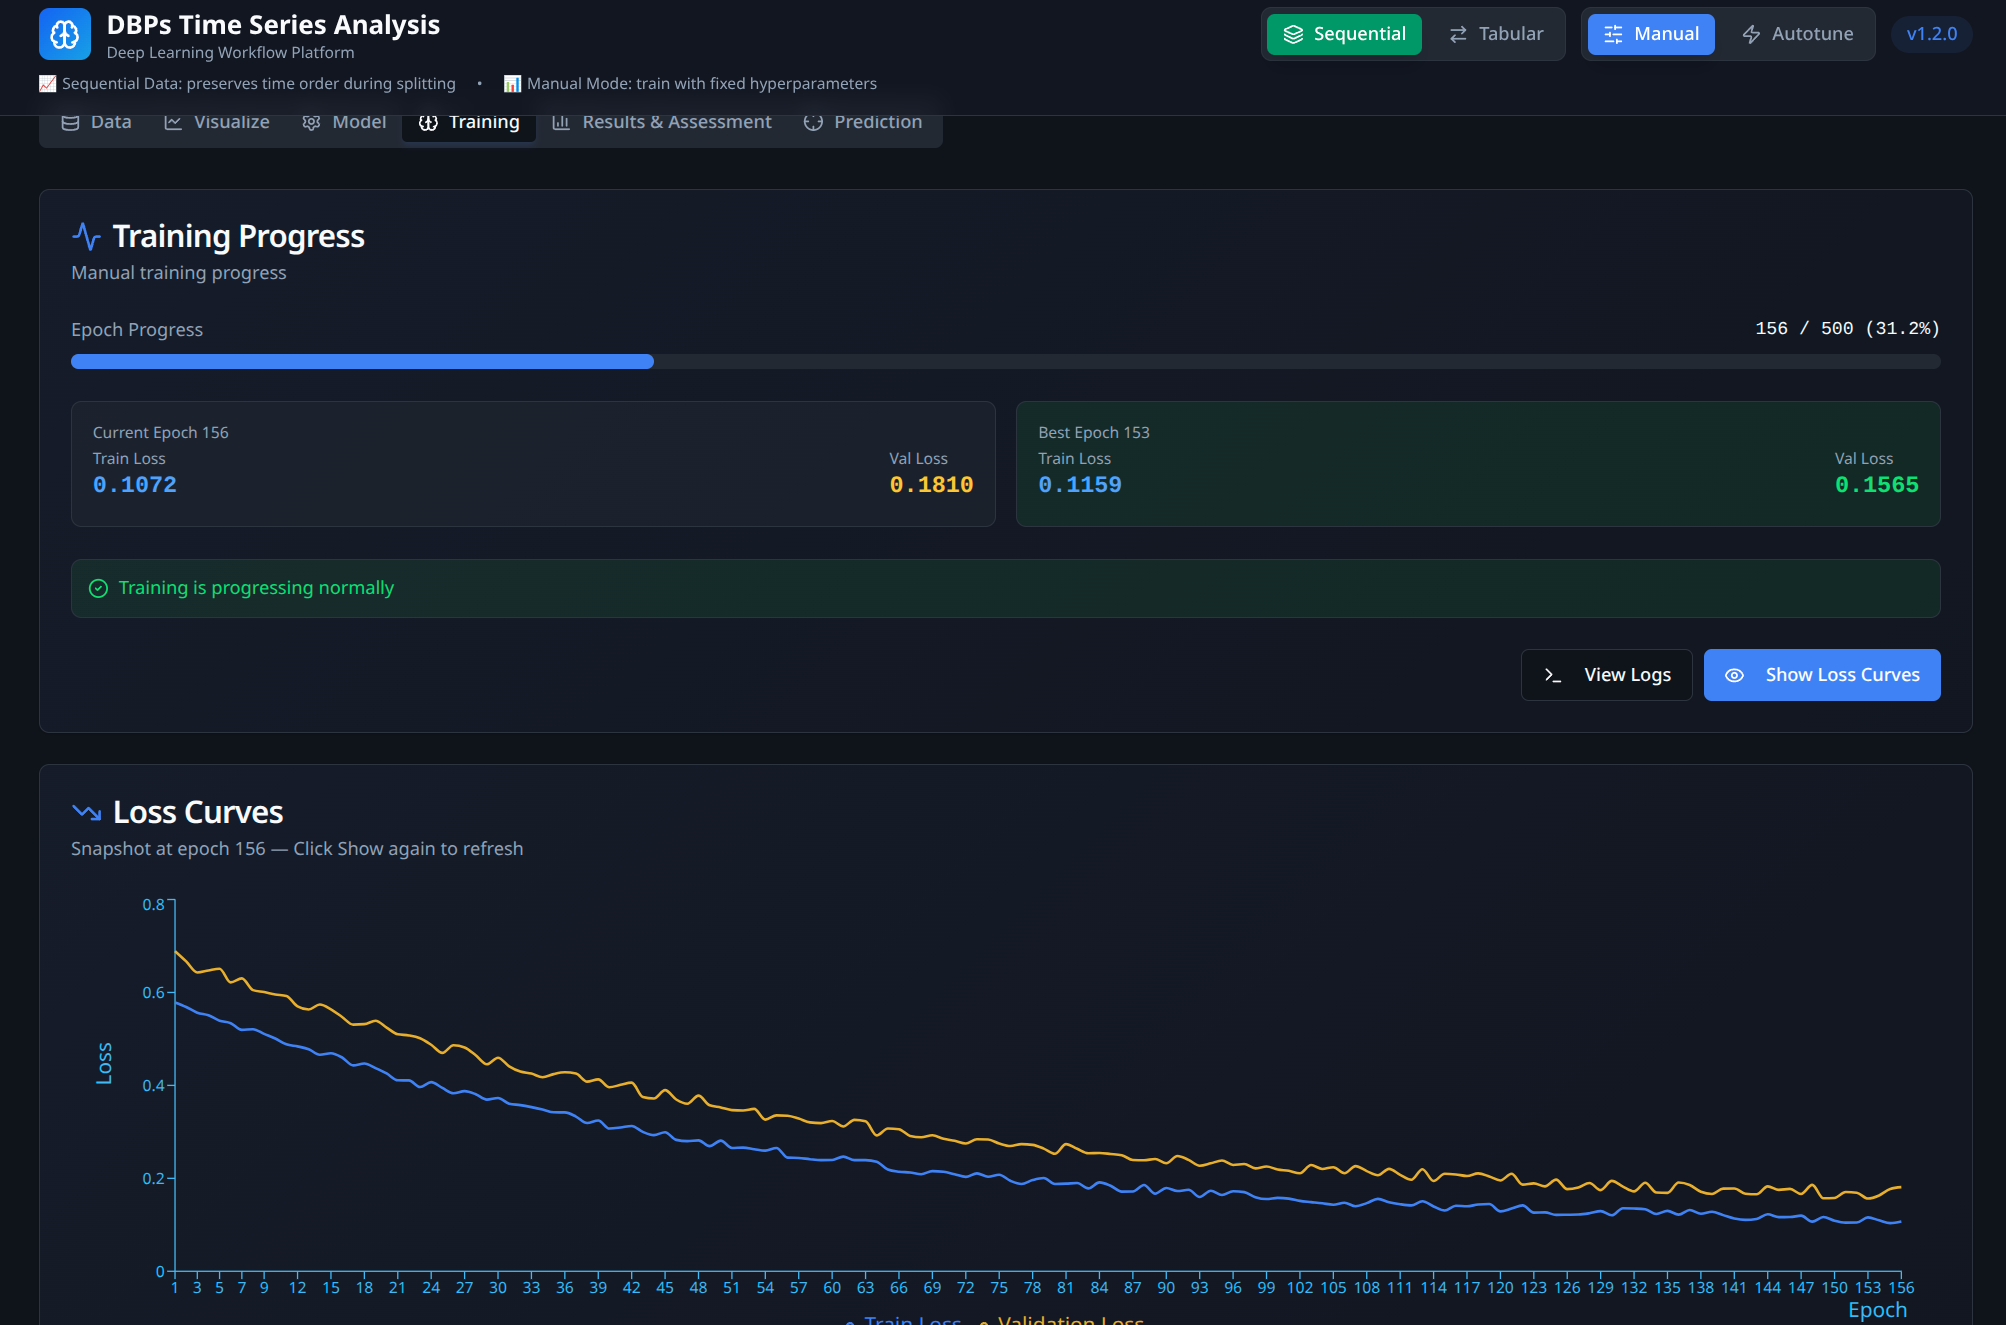
\includegraphics[width=0.9\textwidth]{../attachment/frontend.png}
    \caption{Interactive Graphical User Interface (GUI) of the developed system.}
    \label{fig:frontend}
\end{figure}

The application's decoupled client-server architecture ensures seamless cross-platform functionality (Windows, macOS, Linux) and paves the way for future scalability, enabling the backend to be hosted on high-performance cloud computing clusters while the frontend remains lightweight. This tool has the potential to significantly impact the water treatment industry by democratizing access to cutting-edge predictive models for facility operators.

\section{Future Work}
Based on the progress to date, several future directions have been identified, as outlined in the experimental framework shown in Figure \ref{fig:exp_framework}.
\begin{itemize}
    \item \textbf{Model Interpretability:} Employ interpretability techniques such as SHAP (SHapley Additive exPlanations) and PDP (Partial Dependence Plots) to understand the model's decision-making process. This will help identify which sensor features have the most significant impact on DBP formation predictions.
    \item \textbf{Develop a Second-Stage DBP Model:} Create a subsequent model to establish a mapping from the predicted water quality parameters (TRC, TOC, pH) to actual DBP concentrations measured by offline laboratory instruments, achieving the ultimate goal of predicting specific health-hazardous DBP levels directly from real-time sensors.
\end{itemize}

\begin{figure}[h!]
    \centering
    \includegraphics[width=\textwidth]{../attachment/experiment framework.png}
    \caption{The experimental framework guiding future work.}
    \label{fig:exp_framework}
\end{figure}

\clearpage
\bibliographystyle{unsrt}
\bibliography{references}

\clearpage
\appendix
\section{Appendix: Model Visualization Plots}
\label{app:visualizations}
This appendix provides the comprehensive visual results for the regression performance of both GBDT and Neural Network models, specifically demonstrating the Total Residual Chlorine predictions at Pipeline 2 (TRC-PPL2).

\begin{table}[h!]
    \centering
    \caption{Visualized Performance of TRC-PPL2 for GBDT Models.}
    \label{tab:gbdt_plots}
    \resizebox{\textwidth}{!}{
    \begin{tabular}{|c|c|c|}
        \hline
        \textbf{Model} & \textbf{Prediction vs. True Plot} & \textbf{Y=X Scatter Plot} \\
        \hline
        \textbf{XGBoost} &
        \begin{minipage}{0.4\textwidth}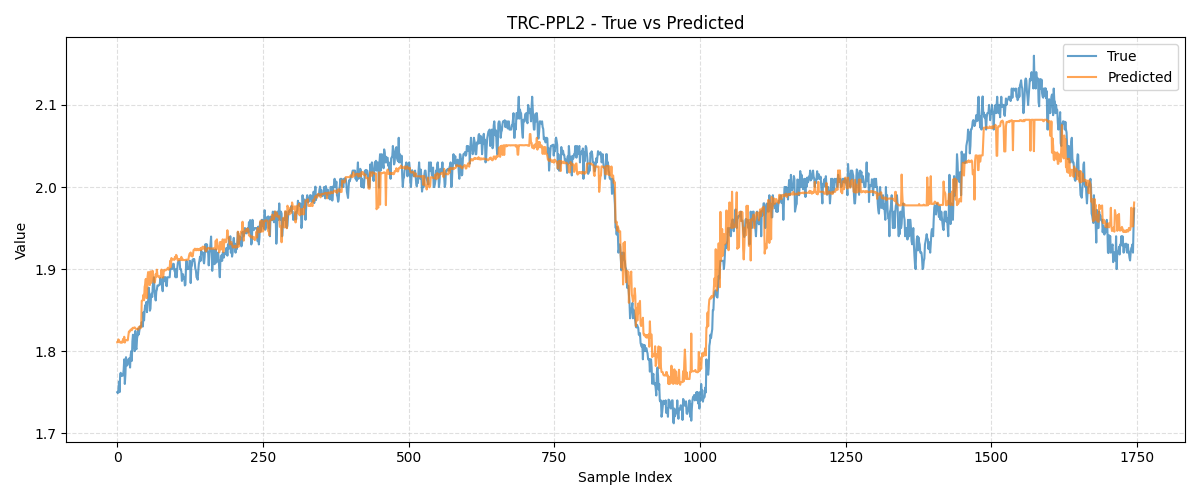
\includegraphics[width=\linewidth]{../../Archived/final-results/caww29-results/xgboost/test_results/TRC-PPL2_pred_vs_true.png}\end{minipage} &
        \begin{minipage}{0.4\textwidth}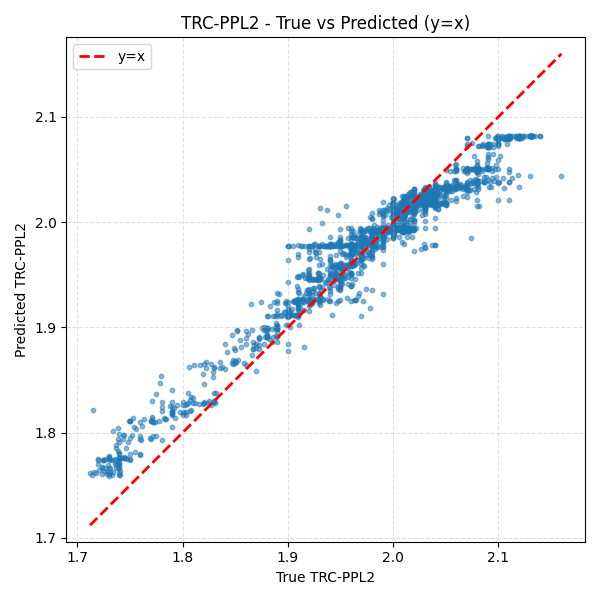
\includegraphics[width=\linewidth]{../../Archived/final-results/caww29-results/xgboost/test_results/TRC-PPL2_yx_scatter.png}\end{minipage} \\
        \hline
        \textbf{LightGBM} &
        \begin{minipage}{0.4\textwidth}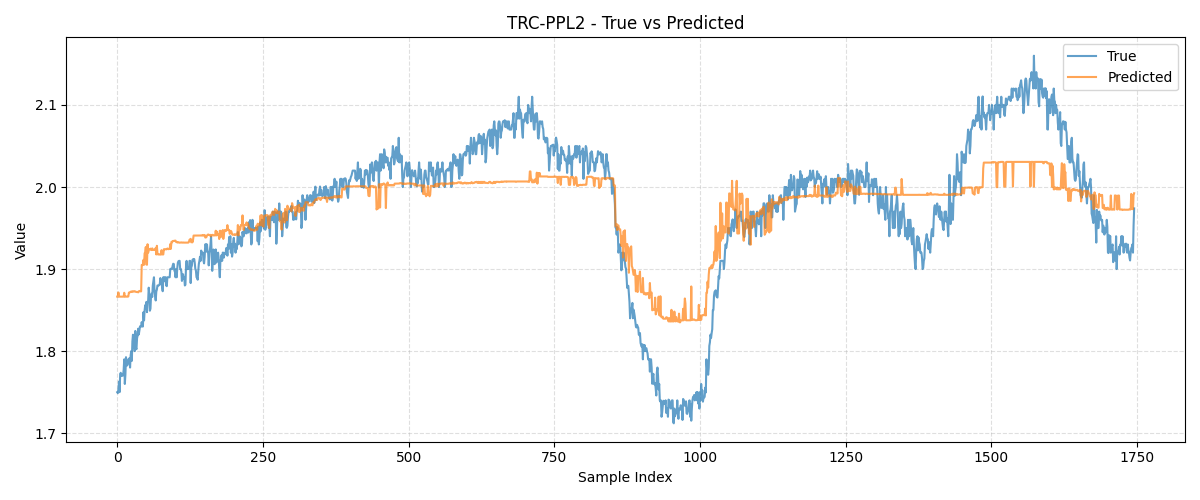
\includegraphics[width=\linewidth]{../../Archived/final-results/caww29-results/lightgbm/test_results/TRC-PPL2_pred_vs_true.png}\end{minipage} &
        \begin{minipage}{0.4\textwidth}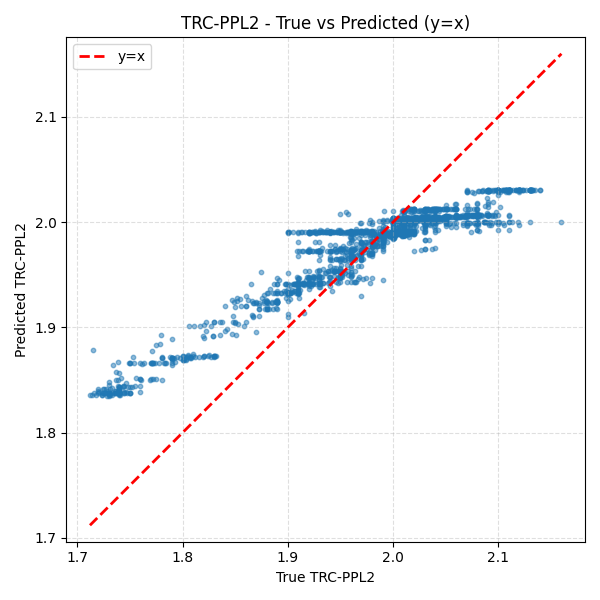
\includegraphics[width=\linewidth]{../../Archived/final-results/caww29-results/lightgbm/test_results/TRC-PPL2_yx_scatter.png}\end{minipage} \\
        \hline
        \textbf{CatBoost} &
        \begin{minipage}{0.4\textwidth}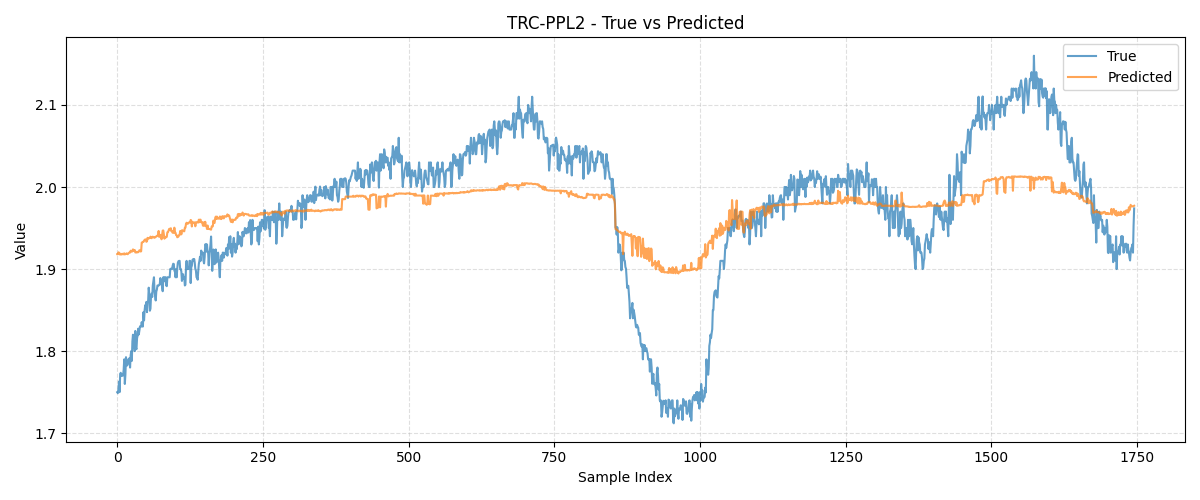
\includegraphics[width=\linewidth]{../../Archived/final-results/caww29-results/catboost/test_results/TRC-PPL2_pred_vs_true.png}\end{minipage} &
        \begin{minipage}{0.4\textwidth}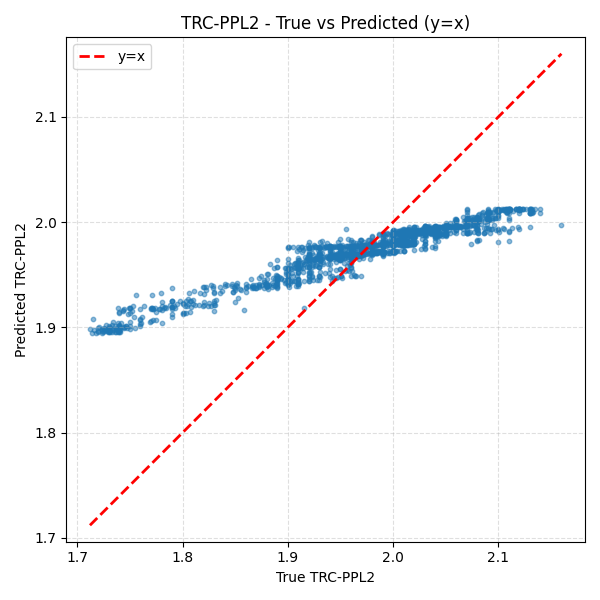
\includegraphics[width=\linewidth]{../../Archived/final-results/caww29-results/catboost/test_results/TRC-PPL2_yx_scatter.png}\end{minipage} \\
        \hline
    \end{tabular}
    }
\end{table}

\begin{table}[h!]
    \centering
    \caption{Visualized Performance of TRC-PPL2 for NN Models (Part 1).}
    \label{tab:nn_plots_1}
    \resizebox{\textwidth}{!}{
    \begin{tabular}{|c|c|c|}
        \hline
        \textbf{Model} & \textbf{Prediction vs. True Plot} & \textbf{Y=X Scatter Plot} \\
        \hline
        \textbf{MLP} &
        \begin{minipage}{0.4\textwidth}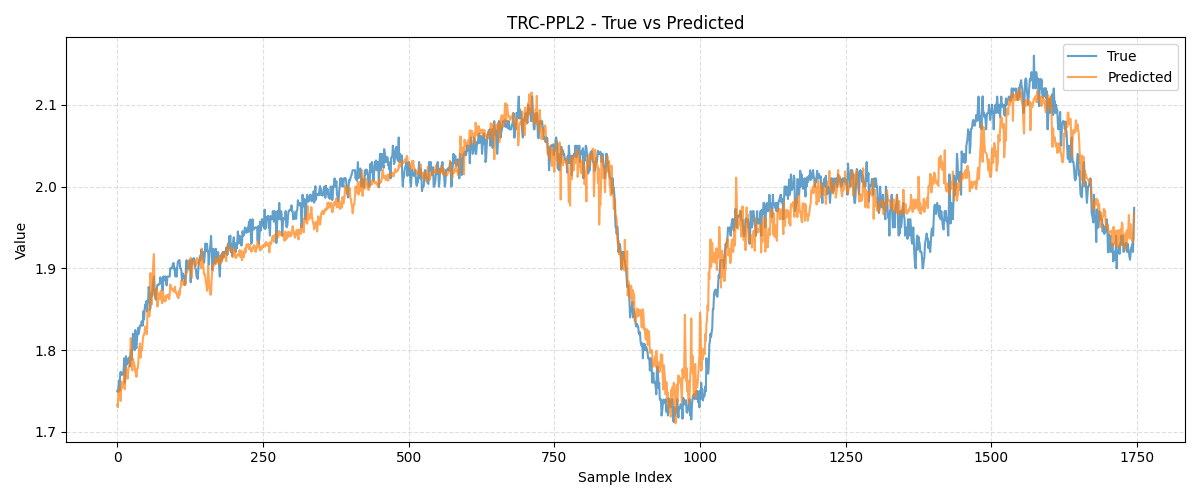
\includegraphics[width=\linewidth]{../../Archived/final-results/caww29-results/mlp/test_results/TRC-PPL2_pred_vs_true.png}\end{minipage} &
        \begin{minipage}{0.4\textwidth}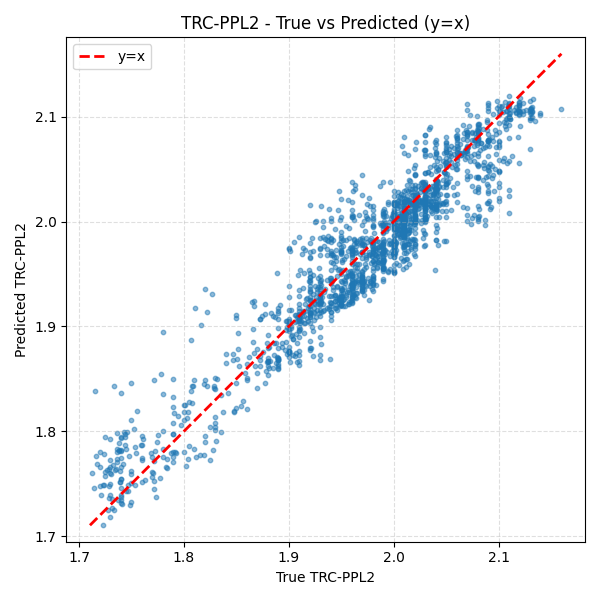
\includegraphics[width=\linewidth]{../../Archived/final-results/caww29-results/mlp/test_results/TRC-PPL2_yx_scatter.png}\end{minipage} \\
        \hline
        \textbf{RNN} &
        \begin{minipage}{0.4\textwidth}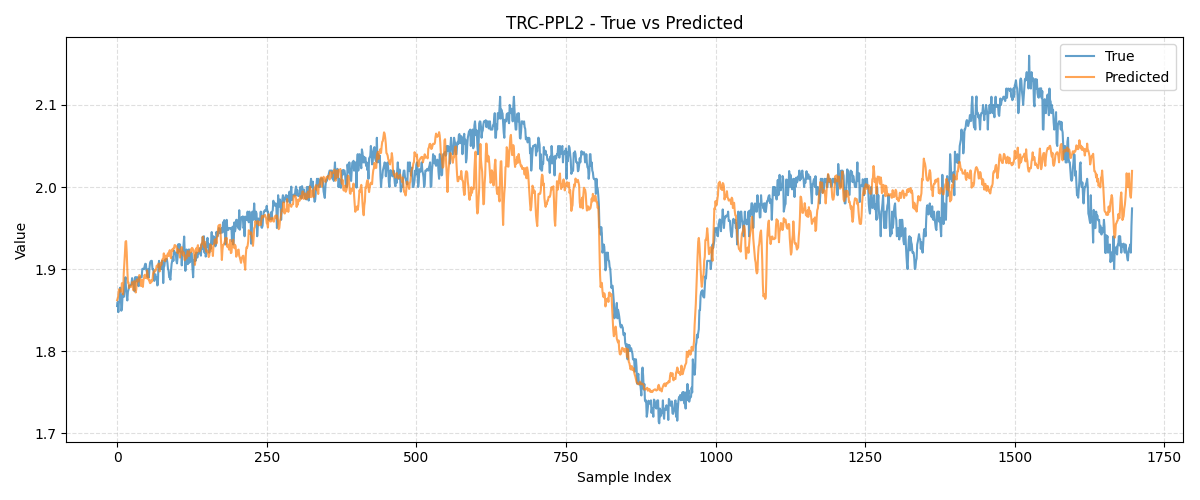
\includegraphics[width=\linewidth]{../../Archived/final-results/caww29-results/rnn/test_results/TRC-PPL2_pred_vs_true.png}\end{minipage} &
        \begin{minipage}{0.4\textwidth}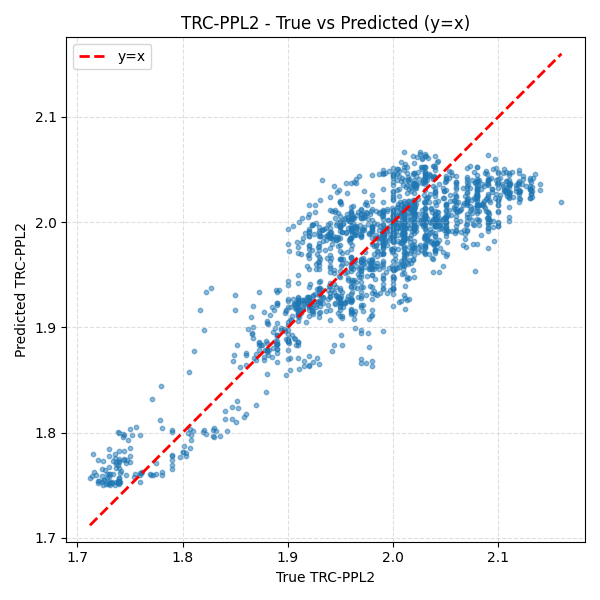
\includegraphics[width=\linewidth]{../../Archived/final-results/caww29-results/rnn/test_results/TRC-PPL2_yx_scatter.png}\end{minipage} \\
        \hline
        \textbf{GRU} &
        \begin{minipage}{0.4\textwidth}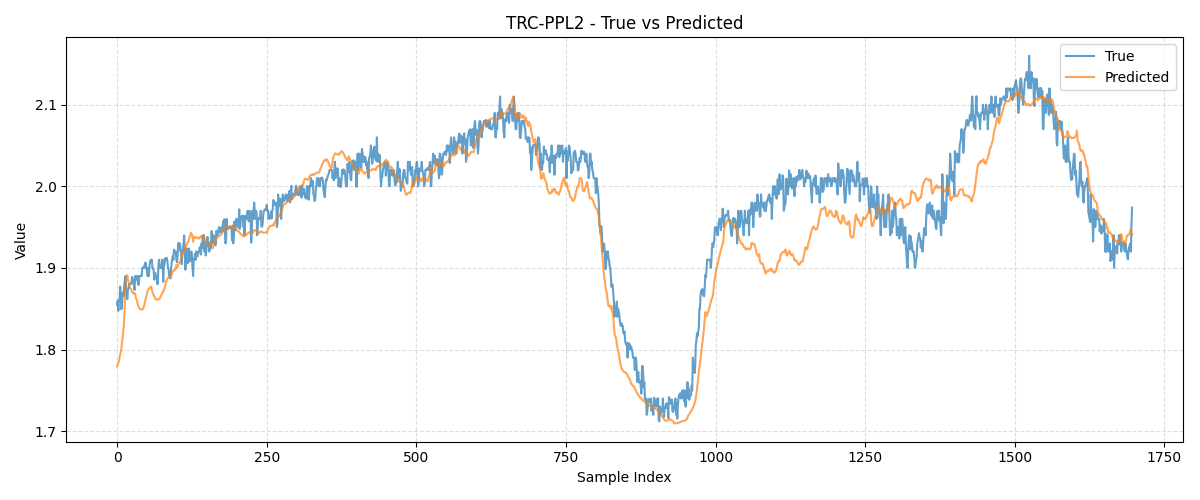
\includegraphics[width=\linewidth]{../../Archived/final-results/caww29-results/gru/test_results/TRC-PPL2_pred_vs_true.png}\end{minipage} &
        \begin{minipage}{0.4\textwidth}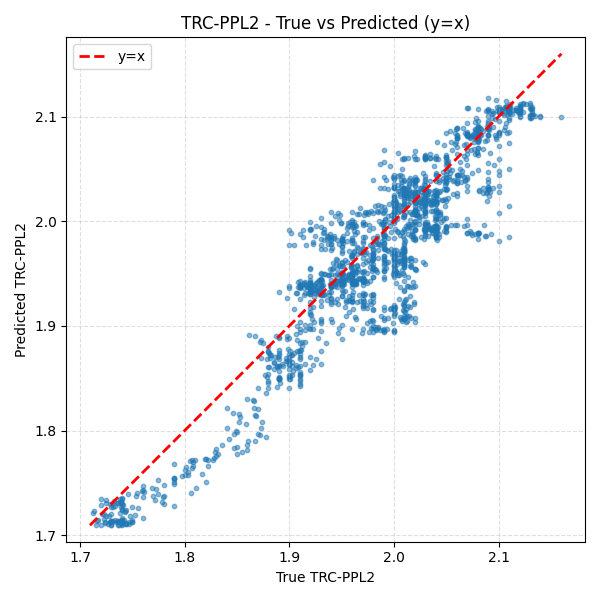
\includegraphics[width=\linewidth]{../../Archived/final-results/caww29-results/gru/test_results/TRC-PPL2_yx_scatter.png}\end{minipage} \\
        \hline
    \end{tabular}
    }
\end{table}

\begin{table}[h!]
    \centering
    \caption{Visualized Performance of TRC-PPL2 for NN Models (Part 2).}
    \label{tab:nn_plots_2}
    \resizebox{\textwidth}{!}{
    \begin{tabular}{|c|c|c|}
        \hline
        \textbf{Model} & \textbf{Prediction vs. True Plot} & \textbf{Y=X Scatter Plot} \\
        \hline
        \textbf{LSTM} &
        \begin{minipage}{0.4\textwidth}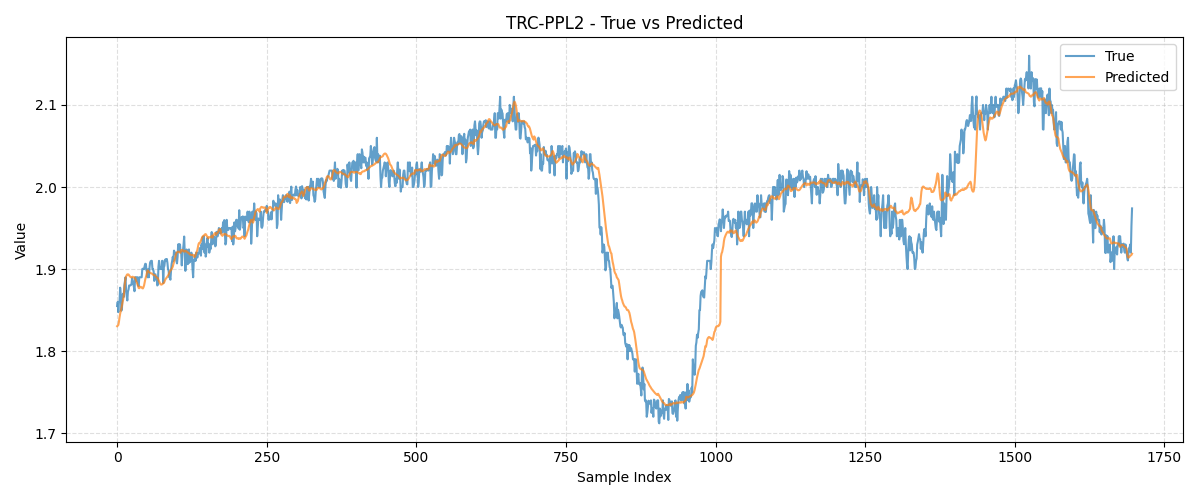
\includegraphics[width=\linewidth]{../../Archived/final-results/caww29-results/lstm/test_results/TRC-PPL2_pred_vs_true.png}\end{minipage} &
        \begin{minipage}{0.4\textwidth}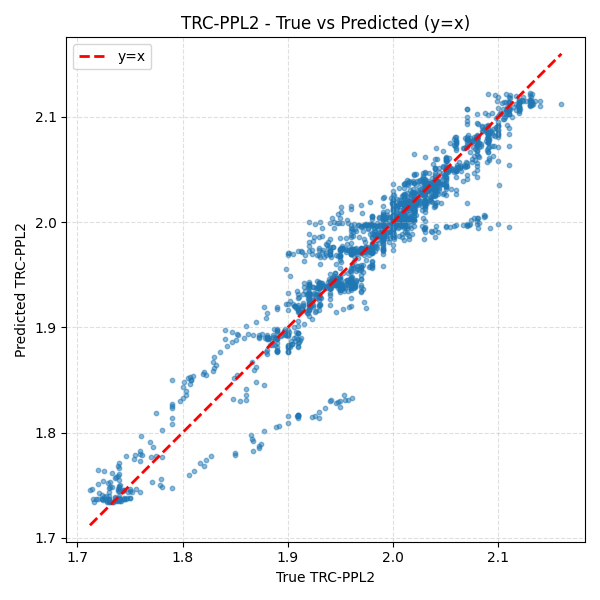
\includegraphics[width=\linewidth]{../../Archived/final-results/caww29-results/lstm/test_results/TRC-PPL2_yx_scatter.png}\end{minipage} \\
        \hline
        \textbf{Transformer} &
        \begin{minipage}{0.4\textwidth}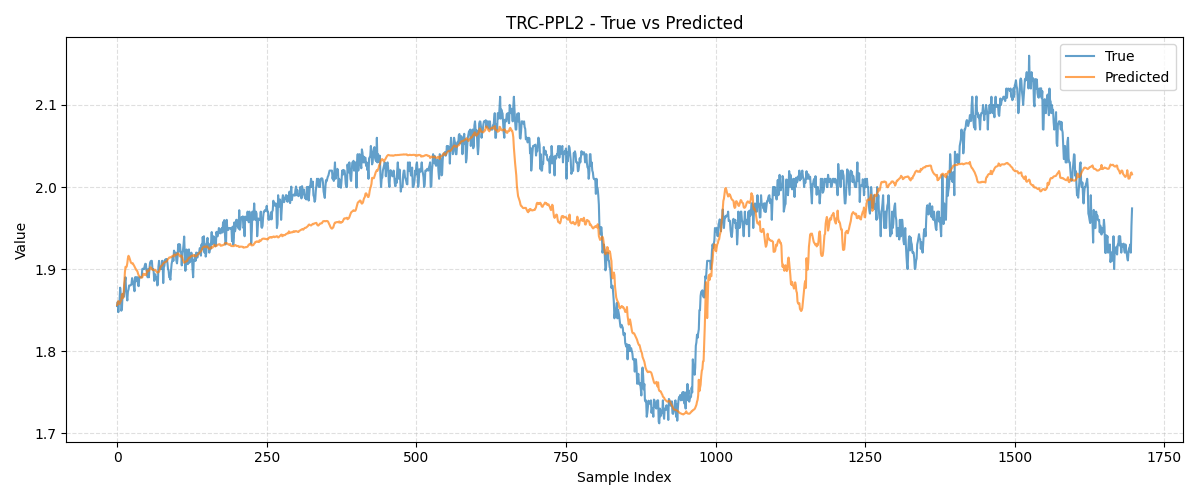
\includegraphics[width=\linewidth]{../../Archived/final-results/caww29-results/transformer/test_results/TRC-PPL2_pred_vs_true.png}\end{minipage} &
        \begin{minipage}{0.4\textwidth}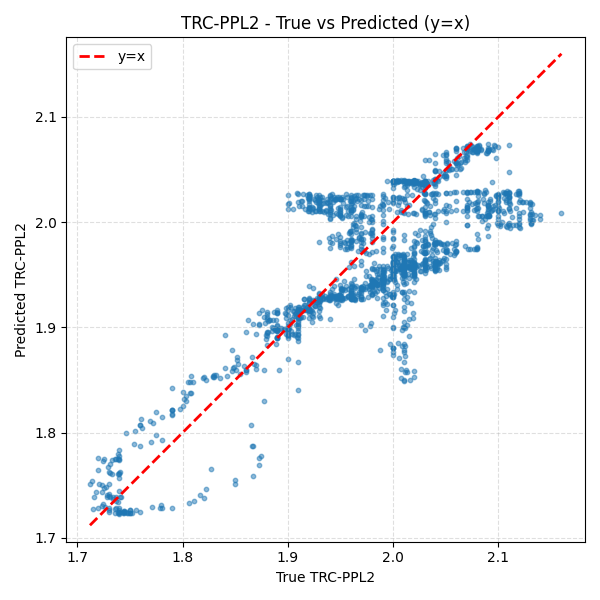
\includegraphics[width=\linewidth]{../../Archived/final-results/caww29-results/transformer/test_results/TRC-PPL2_yx_scatter.png}\end{minipage} \\
        \hline
        \textbf{Mamba} &
        \begin{minipage}{0.4\textwidth}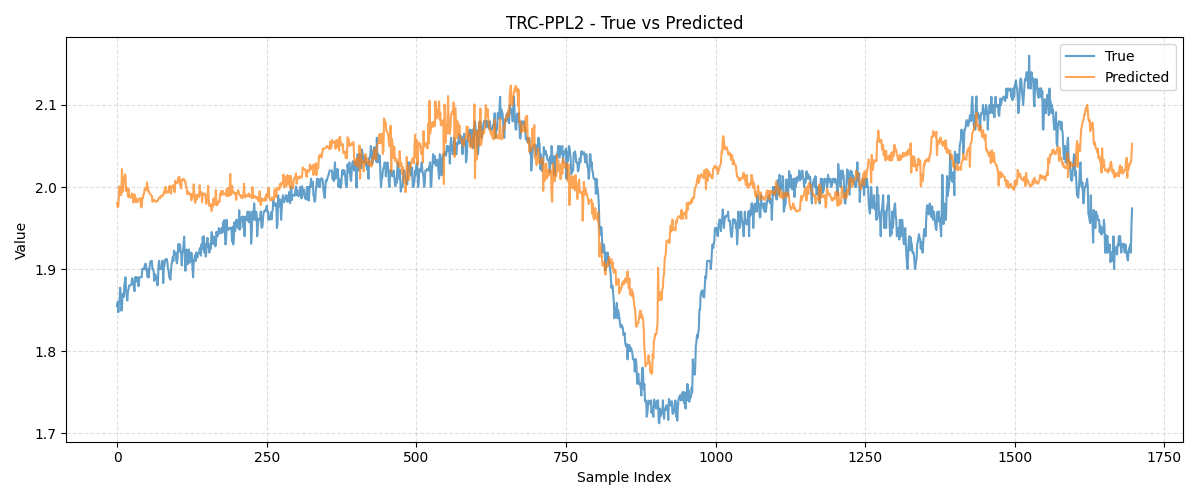
\includegraphics[width=\linewidth]{../../Archived/final-results/caww29-results/mamba/test_results/TRC-PPL2_pred_vs_true.png}\end{minipage} &
        \begin{minipage}{0.4\textwidth}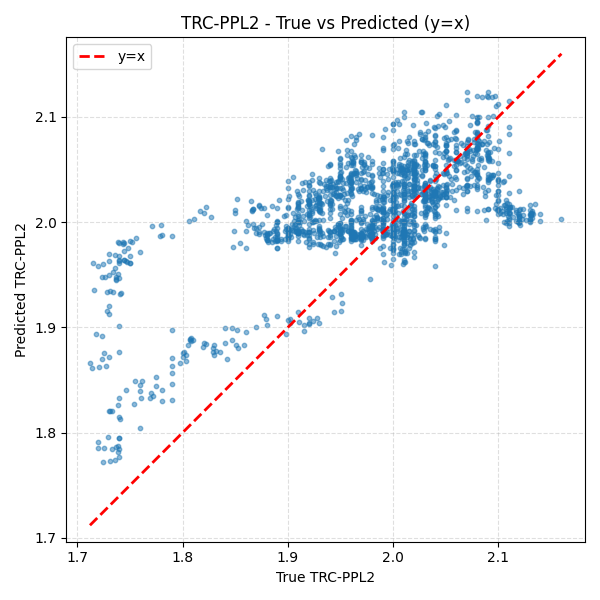
\includegraphics[width=\linewidth]{../../Archived/final-results/caww29-results/mamba/test_results/TRC-PPL2_yx_scatter.png}\end{minipage} \\
        \hline
    \end{tabular}
    }
\end{table}

\end{document}
